\chapter{System Setup}

\section{Overview}
%How do we define the solution?
%	Combined solution 
%	Link between
%	Physical setup/limitations

To make an emulator, that can emulate all scenarios for NB-IoT compared to the test domains, chosen in \todo{ref to domain selection}, a setup, shown on figure \todo{ref}, is chosen. This setup contains a \gls{eNB}, the possibility to connect external IoT devices and the components need to emulate and analyze the test scenarios from the domains. All the components in the emulator, is software based, but are connected together through wires.

\todo{Insert beautiful figure}


%First, there should be a conceptual diagram of the setup; this should go into a description of how the emulator is actually put together. 
%There should be a mention of how an external device can be put into the system to be tested also due to the cellular nature of NB-IoT.
%The physical connection needs to be explained, how to connect everything and where to put attenuators combiners and so forth.
%There could also be a section of practical limitation due to digitalization.
%Should end with differentiation of main and auxiliary components.

%\begin{figure}[H]
%\centering
%\resizebox{0.5\textwidth}{!}{
%\begin{tikzpicture}[scale=0.15]


\draw  (-10,15) rectangle (10,5);
\node at (0,10) {Orchestrator};

\draw  (-40,0) rectangle (-20,-10);
\node at (-30,-5) {PSU};

\draw  (-10,0) rectangle (10,-10);
\node at (0,-5) {Ext. Device};

\draw  (20,0) rectangle (40,-10);
\node at (30,-5) {eNB};

\draw  (-10,-15) rectangle (10,-25);
\node at (0,-20) {Massive IoT};

\node(PSU_top) at (-30,0) {};
\node(PC_left) at (-10,12) {};
\node(PC_bot) at (0,5) {};
\node(DUT_top) at (0,0) {};
\node(PC_right) at (10,10) {};
\node(eNB_top) at (30,0) {};
\node(v1) at (-30,12) {};
\node(v2) at (30,10) {};
\node(PSU_left) at (-20,-5) {};
\node(PC_left2) at (-10,8) {};
\node(DUT_left) at (-10,-5) {};
\node(DUT_right) at (10,-5) {};
\node(eNB_left) at (20,-5) {};

\draw (-10,12) -- (-30,12) -- (-30,0);
\draw (10,10) -- (30,10) -- (30,0);
\draw  (0,5) -- (0,0);
\draw  (-20,-5) -- (-10,-5);
\draw  (10,-5) -- (20,-5);

%[arrows={ - triangle 45}] 
\draw (-10,8) -- (-15,8) -- (-15,-20) -- (-10,-20);

\draw (10,-20) -- (30,-20) -- (30,-10);
\end{tikzpicture}

}
%\caption{Testbed overview}
%\label{fig:test-bed_overview}
%\end{figure}

\textbf{eNB}\\

To emulate a cellular network for this project, a \gls{BS} is needed, which supports \gls{NB-IoT}. As it is not the BS that are in testing focus for this emulator, there can be use an already existing \gls{BSE}. The BSE should be changeable, with the only connections to the system being a physical wired connection to the NB-IoT devices and a control input from the Orchestrator.

For emulation of the massiveness part, the Amarisoft LTE 100 code will be used as it can handle 1000 \gls{UE} \todo{Insert ref to Amarisoft side} and is tested to synchronize with the software based NB-IoT devices from the Massive IoT component. As it is a commercial BSE, it is not open source and therefore harder to add new features and see all parameters for, so it will only be used for the massiveness part in this project.

For emulation of the battery life part, the \gls{UXM} will be used as it is a test equipment and therefore designed to be able to change all parameters and get output data from. Unfortunately is it not designed to a higher amount of UE and can not be used for the massiveness part.

%Here should be mentioned that the BSE is not primary concern, therefore use of exsiting BSE. It should also be mentioned that it should be changeable so commercial BS can also be tested. It should end with use we use Amarisoft LTE 100 as primary and support it with UXM.
%	Amarisoft
%Here should be a list of relevant features it have, and how to use them. It should also be mentioned, how we can access it from a main PC to set these features. It should be described how the core network interacts with the eNB. It should also be described where to put USIM data to allow network attach.
%	UXM
%	Here should be a list of relevant features it have, and how to use them. It should also be mentioned, how we can access it from a main PC to set these features. It should be described how the core network interacts with the eNB. It should also be described where to put USIM data to allow network attach.

\textbf{Massive IoT}\\
To emulate a massive amount of NB-IoT devices to stress test the BS and to interfere with the external NB-IoT device, a software base solution is selected. The ground block for the solution is the SRS NB-IoT UE code, provide by \todo{Can we mention keysight here}, where the code have to be modified to produce multiple UE compared to the single it produce as standard.

%Here should be a description of the software from SRS. How the core structure of the code is and how it is expanded to accommodate multiple UEs. There should be a description of how to change key parameters in the code and how to use the system from a main PC (or if the main PC should host the MassM2M).

\textbf{PSU}\\
To provide and measure the power use by external NB-IoT device a \gls{PSU} is use. By having the external device connected to the PSU, the power used in different scenarios can be measured. In this case a \todo{Name the fucking equipment} is used as it can be hooked up to the Orchestrator that are being used in these scenarios.
%Short description of the feature of the PSU and the limitation (can not measure and change settings simultaneously). There should also be a description of how the PSU responds to SCIPI commands.

\textbf{External device}\\
The possibility for connecting an external NB-IoT device, will make it possible to test different scenarios compared to the individual UE handle the massiveness, produce by the Massive IoT component, and measure the battery life, as different devices will have different battery life.
%An explanation of why it is nice to include (possibility to test commercial devices). Some examples of commercial devices. 

\textbf{Orchestrator}\\
To control the whole emulator, an orchestrator is wanted to control the emulator and handle in- and outputs. The PSU and the UXM used for the battery life test is already set up to be handle with the program called \todo{Thomas, talk about the wonders of TAP}

The code for the Massive IoT is started up on is own and gets its parameter from a config file. 
%What are the function of the orchestrator? Mention the use of TAP. A list of all connections and communication protocols. 



%\section{Massiveness}
%%	What features?
%%	What have we changed/done?
%
%\section{Energy}
%%	What features?
%%	What have we changed/done?
%
%With the \gls{NB-IoT} protocol explained it is time to look into the design of the \gls{IoT} emulator. The general idea is to make the following system. 
%
%\begin{figure}[H]
%\centering
%\resizebox{0.8\textwidth}{!}{
%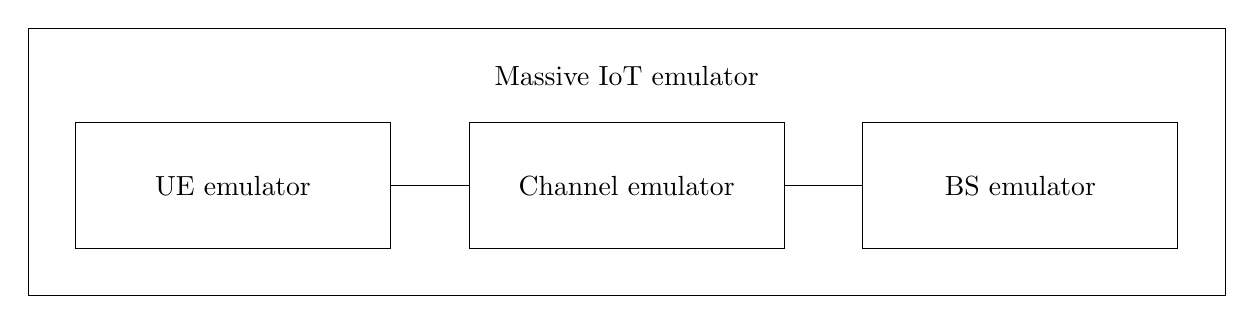
\begin{tikzpicture}[scale=0.2]

\draw  (-38,14) rectangle (38,-3);
\node at (0,11) {Massive IoT emulator};

\draw  (-35,8) rectangle (-15,0);
\node at (-25,4) {UE emulator};

\draw  (-10,8) rectangle (10,0);
\node at (0,4) {Channel emulator};

\draw  (35,8) rectangle (15,0);
\node at (25,4) {BS emulator};

\draw (-15,4) -- (-10,4);

\draw (10,4) -- (15,4);
\end{tikzpicture}}
%\caption{emulator overview}
%\label{fig:emulator_overview}
%\end{figure}
%
%The \gls{UEE} will be connected to the \gls{BSE} through a cable, this will remove the interference to and thereby the restriction of using licensed the licensed spectrum. This also means it would be advantageous to move the channel emulator to either the \gls{UEE} or the \gls{BSE}. 
%
%As mentioned in \autoref{ch:Introduction} the task is quite huge, therefore is it necessary to use existing software when possible and use experiences from earlier work in this field.
%
%
%\section{Earlier work}
%A similar system has been built before in 2017 by Mathias Kielgast and Anders Rasmussen \citep{thesis_report}. They used two \gls{SDR}s to emulate a basestation and multiple \gls{LTE} devices respectively. They took the existing srsUE system and changed the structure to handle multiple UEs. The design principle, as can also been seen in \autoref{fig:thesis_structure}, is to emulate multiple \gls{LTE} protocol stacks in which is connected to a commen physical layer. This allows for the multiple devices to be independent from each other, but still using the same \gls{SDR}. \citep{thesis_report} 
%
%\begin{figure}[H]
%\centering
%\includegraphics[width=0.7\textwidth]{figures/thesis_structure.png}
%\caption{thesis structure \citep{thesis_report}}
%\label{fig:thesis_structure}
%\end{figure}
%
%
%The system was made to prove if the method could work for a \gls{MTC} type of connection also. In this way they made a proof of concept product that emulated 15 devices using a 5 MHz bandwidth. They also proved that smaller bandwidth allowed the system to emulate more devices. The UEE used the the srsUE as a framework while the BSE used the \gls{OAI}. \citep{thesis_report} 
%
%The design of the \gls{MITE} relies heavily on the work done in this project. However as it is intended to use the \gls{NB-IoT} protocol instead of \gls{LTE} it is necessary to use another version of srsUE as well as another framework entirely for the \gls{BS} emulator. The \gls{BS} emulator will instead rely on the Amarisoft BSE.
%
%%\section{General Setup}
%\section{Basestation emulator}
%As found in the \autoref{ch:Introduction} there is two possibilities when choosing the \gls{BSE}, Amairsoft and SRS. It has been chosen to work with the Amarisoft \gls{BSE}, as it provides the necessary features and comes with support. The SRS \gls{BSE} is not yet fully developed so it might require a lot more time to get working. Another alternative altogether is the Keysight E7515A UXM, it also provides the needed features it is just a lot more expensive. Therefore the \gls{BSE} chosen is the Amarisoft LTE 100.
%
%Amarisoft LTE 100 features LTE, LTE-A, LTE-M and NB-IoT protocols.    For the NB-IoT protocol it specifically features\citep{Amarisoft_solutions}:
%
%\begin{itemize}
%\item NB-IoT release 14 compliant
%\item Single-tone and multi-tone category NB1 and NB2 UE support
%\item 15 kHz and 3.75 kHz subcarrier spacing are supported
%\item All operation modes (in-band, guard band and standalone) are supported
%\item Multiple NB-IoT and LTE cells can be used at the same time in the same eNodeB
%\item Support of multiple coverage levels
%\item Support of all NPDCCH, NPDSCH, NPUSCH and NPRACH configurations
%\item Support of control plane CIoT optimization
%\item Support of multi-DRB mode
%\end{itemize}
%
%\section{User Equipment Emulator}
%\subsection{Quectel}
%\subsection{SRS UE}
%
%
% and the channel emulator will be implemented only as a simple \gls{PL} factor. 


